\documentclass{article}

\usepackage{amsmath,amssymb}
\usepackage{tikz}
\usetikzlibrary{er,positioning}
\usepackage{pgfplots}
\usepackage{xcolor}
\usepackage[left=2.1cm,right=3.1cm,bottom=3cm,footskip=0.75cm,headsep=0.5cm]{geometry}
\usepackage{enumerate}
\usepackage{enumitem}
\usepackage{marvosym}
\usepackage{tabularx}

\usepackage{listings}
\definecolor{lightlightgray}{rgb}{0.95,0.95,0.95}
\definecolor{lila}{rgb}{0.8,0,0.8}
\definecolor{mygray}{rgb}{0.5,0.5,0.5}
\definecolor{mygreen}{rgb}{0,0.8,0.26}
\lstdefinestyle{java} {language=java}
\lstset{language=java,
	basicstyle=\ttfamily,
	keywordstyle=\color{lila},
	commentstyle=\color{lightgray},
	stringstyle=\color{mygreen}\ttfamily,
	backgroundcolor=\color{white},
	showstringspaces=false,
	numbers=left,
	numbersep=10pt,
	numberstyle=\color{mygray}\ttfamily,
	identifierstyle=\color{blue},
	xleftmargin=.1\textwidth, 
	%xrightmargin=.1\textwidth,
	escapechar=§,
}

\usepackage[utf8]{inputenc}

\renewcommand*{\arraystretch}{1.4}

\newcolumntype{L}[1]{>{\raggedright\arraybackslash}p{#1}}
\newcolumntype{R}[1]{>{\raggedleft\arraybackslash}p{#1}}
\newcolumntype{C}[1]{>{\centering\let\newline\\\arraybackslash\hspace{0pt}}m{#1}}

\newcommand{\E}{\mathbb{E}}
\DeclareMathOperator{\rk}{rk}
\DeclareMathOperator{\Var}{Var}
\DeclareMathOperator{\Cov}{Cov}

\title{\textbf{Datenbanken, Übung 2}}
\author{\textsc{Henry Haustein}}
\date{}

\begin{document}
	\maketitle
	
	\section*{Aufgabe 1}
	\begin{enumerate}[label=(\alph*)]
		\item ER-Diagramm mit (min, max)-Notation:
		\begin{center}
			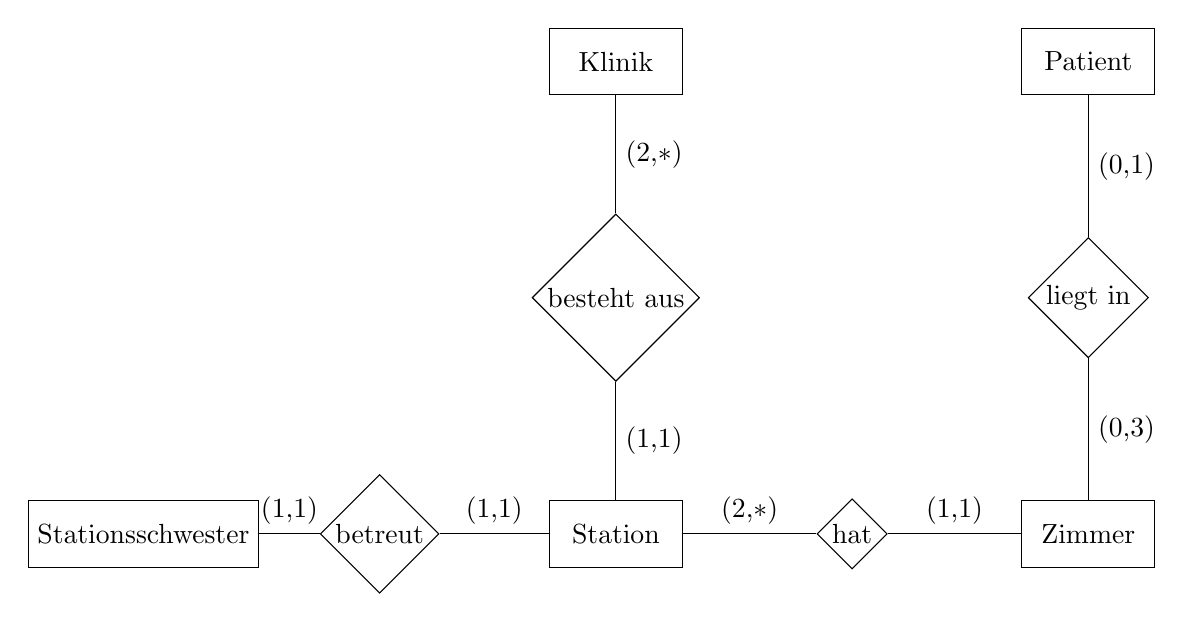
\begin{tikzpicture}
				\node[entity] at (0,0) (ss) {Stationsschwester};
				\node[entity] at (6,0) (s) {Station};
				\node[entity] at (6,6) (k) {Klinik};
				\node[entity] at (12,0) (z) {Zimmer};
				\node[entity] at (12,6) (p) {Patient};
				
				\node[relationship] at (3,0) (b) {betreut};
				\node[relationship] at (6,3) (be) {besteht aus};
				\node[relationship] at (9,0) (h) {hat};
				\node[relationship] at (12,3) (l) {liegt in};
				
				\draw (ss) to node[above] {(1,1)} (b) to node[above] {(1,1)} (s);
				\draw (s) to node[above] {(2,$\ast$)} (h) to node[above] {(1,1)} (z);
				\draw (k) to node[right] {(2,$\ast$)} (be) to node[right] {(1,1)} (s);
				\draw (p) to node[right] {(0,1)} (l) to node[right] {(0,3)} (z);
			\end{tikzpicture}
		\end{center}
		\item ER-Diagramm mit Funktionalitäten:
		\begin{center}
			\begin{tikzpicture}
				\node[entity] at (0,0) (ss) {Stationsschwester};
				\node[entity] at (6,0) (s) {Station};
				\node[entity] at (6,6) (k) {Klinik};
				\node[entity] at (12,0) (z) {Zimmer};
				\node[entity] at (12,6) (p) {Patient};
				
				\node[relationship] at (3,0) (b) {betreut};
				\node[relationship] at (6,3) (be) {besteht aus};
				\node[relationship] at (9,0) (h) {hat};
				\node[relationship] at (12,3) (l) {liegt in};
				
				\draw (ss) to node[above] {1} (b) to node[above] {1} (s);
				\draw (s) to node[above] {1} (h) to node[above] {N} (z);
				\draw (k) to node[right] {1} (be) to node[right] {N} (s);
				\draw (p) to node[right] {N} (l) to node[right] {1} (z);
			\end{tikzpicture}
		\end{center}
		\item Liste an möglichen Attributen für jeden Entity-Typ, Primärschlüssel ist unterstrichen
		\begin{itemize}
			\item Stationsschwester: \underline{PersonalNummer}, Vorname, Name
			\item Station: \underline{Stationsnummer}, Fachgebiet
			\item Klinik: \underline{Name}, Adresse, Telefonnummer
			\item Patient: \underline{Patientennummer}, Alter, Name, Geschlecht, Symptome
			\item Zimmer: \underline{Zimmernummer}, AnzahlBetten
		\end{itemize}
		\item Dass Frauen und Männer nicht in ein Zimmer dürfen, sowie, dass es keine Zweibettzimmer gibt.
	\end{enumerate}

	\section*{Aufgabe 2}
	Die Relationen sind Mengen mit Elementen der folgenden Form: $(x,y)$ wobei $x\in X$ und $y\in Y$:
	\begin{itemize}
		\item $R_1=\{(6,4),(8,4),(10,4),(10,8)\}$
		\item $R_2=\{(4,4),(8,4),(8,8)\}$
		\item $R_3=\{(2,4),(4,4),(2,8),(4,8),(6,8),(8,8)\}$
	\end{itemize}
	Damit ergibt sich folgendes ER-Diagramm
	\begin{center}
		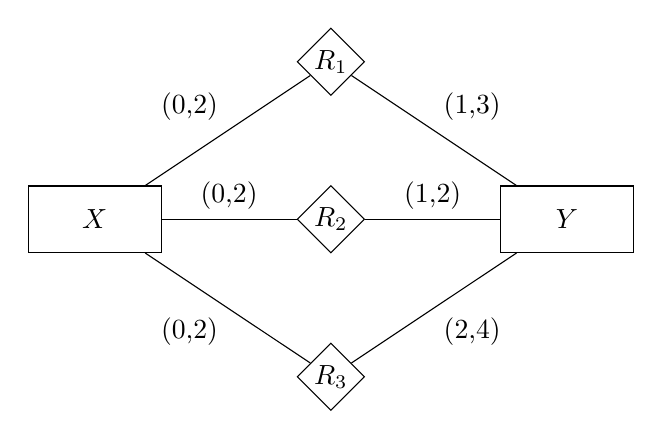
\begin{tikzpicture}
			\node[entity] at (0,0) (x) {$X$};
			\node[entity] at (6,0) (y) {$Y$};
			
			\node[relationship] at (3,2) (r1) {$R_1$};
			\node[relationship] at (3,0) (r2) {$R_2$};
			\node[relationship] at (3,-2) (r3) {$R_3$};
			
			\draw (x) to node[above left] {(0,2)} (r1) to node[above right] {(1,3)} (y);
			\draw (x) to node[above] {(0,2)} (r2) to node[above] {(1,2)} (y);
			\draw (x) to node[below left] {(0,2)} (r3) to node[below right] {(2,4)} (y);
		\end{tikzpicture}
	\end{center}

	\section*{Aufgabe 3}
	\begin{enumerate}[label=(\alph*)]
		\item $A\times B\to C$, $A\times C\to B$ und $B\times C\to A$
		\item Student $\times$ Übung $\to$ Tutor, Tutor $\times$ Student $\to$ Übung und Tutor $\times$ Übung $\to$ Student
		\item Es gilt:
		\begin{itemize}
			\item Tutor $\times$ Übung $\to$ Student: Pro Übung darf ein Tutor nur einen Studenten haben.
			\item Tutor $\times$ Student $\to$ Übung: Ein Student darf bei einem Tutor nur eine Übung besuchen.
			\item Übung $\times$ Student $\to$ Tutor: Es darf pro konkreter Übung nur einen Tutoren geben.
		\end{itemize}
		\item Es gelten alle partiellen Funktionen aus (c), außer Tutor $\times$ Übung $\to$ Student
	\end{enumerate}
	
	\section*{Aufgabe 4}
	Die Funktionalitätsangaben sind
	\begin{center}
		\begin{tikzpicture}
			\node[entity] at (-3,0) (a) {A};
			\node[entity] at (3,0) (b) {B};
			\node[entity] at (0,-2) (c) {C};
			
			\node[relationship] at (0,0) (r) {R};
			
			\draw (a) to node[above] {M} (r);
			\draw (b) to node[above] {1} (r);
			\draw (c) to node[right] {N} (r);
		\end{tikzpicture}
	\end{center}
	Entitäten aus der rechten Seite einer partiellen Funktion werden im ER-Diagramm mit 1 beschriftet.
	
	\section*{Aufgabe 5}
	Die (min,max)-Notationen sind
	\begin{center}
		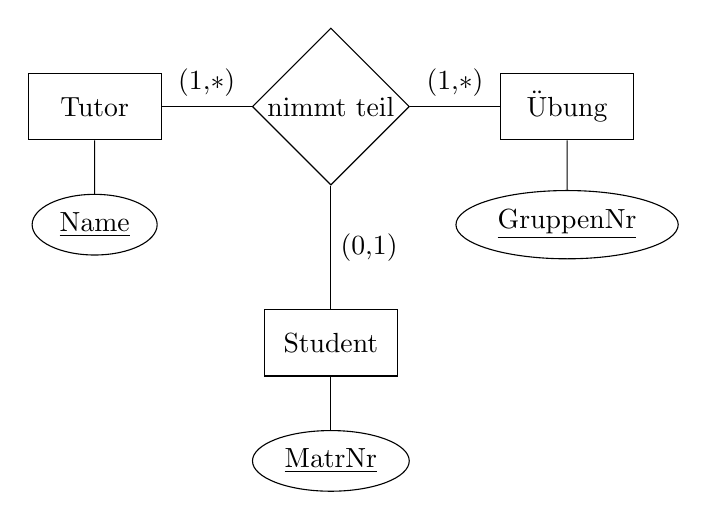
\begin{tikzpicture}
			\node[entity] at (-3,0) (a) {Tutor}
				child {node[attribute] {\underline{Name}}};
			\node[entity] at (3,0) (b) {Übung}
				child {node[attribute] {\underline{GruppenNr}}};
			\node[entity] at (0,-3) (c) {Student}
				child {node[attribute] {\underline{MatrNr}}};
			
			\node[relationship] at (0,0) (r) {nimmt teil};
			
			\draw (a) to node[above] {(1,$\ast$)} (r);
			\draw (b) to node[above] {(1,$\ast$)} (r);
			\draw (c) to node[right] {(0,1)} (r);
		\end{tikzpicture}
	\end{center}
	Die (min,max)-Notation ist genau die minimalen und maximalen Vorkommnisse der Entität in der Tabelle.
	
	\section*{Aufgabe 6}
	Das ER-Diagramm
	\begin{center}
		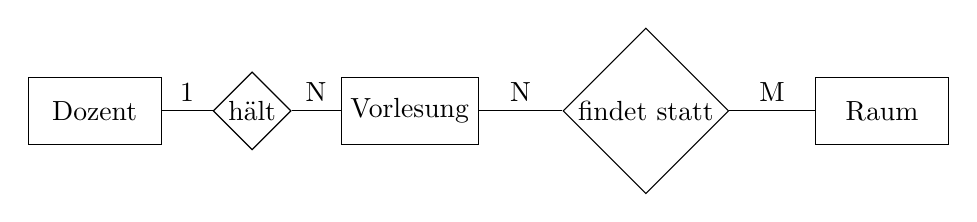
\begin{tikzpicture}
			\node[entity] at (0,0) (d) {Dozent};
			\node[entity] at (4,0) (v) {Vorlesung};
			\node[entity] at (10,0) (r) {Raum};
			
			\node[relationship] at (2,0) (h) {hält};
			\node[relationship] at (7,0) (f) {findet statt};
			
			\draw (d) to node[above] {1} (h) to node[above] {N} (v);
			\draw (v) to node[above] {N} (f) to node[above] {M} (r);
		\end{tikzpicture}
	\end{center}
	
\end{document}